\documentclass[journal]{IEEEtran}
\usepackage[a5paper, margin=10mm, onecolumn]{geometry}
\usepackage{lmodern}

\setlength{\headheight}{1cm}
\setlength{\headsep}{0mm}

\usepackage{gvv-book}
\usepackage{gvv}
\usepackage{cite}
\usepackage{amsmath,amssymb,amsfonts,amsthm}
\usepackage{graphicx}
\graphicspath{{./figs/}}
\usepackage{xcolor}
\usepackage{txfonts}
\usepackage{enumitem}
\usepackage{mathtools}
\usepackage{hyperref}
\usepackage{tikz}
\usepackage{tkz-euclide}

\begin{document}

\bibliographystyle{IEEEtran}
\vspace{3cm}

\title{4.7.34}
\author{EE25BTECH11036 - M Chanakya Srinivas}
\maketitle

\renewcommand{\thetable}{\theenumi}
\setlength{\intextsep}{10pt}
\renewcommand\theequation{\arabic{equation}}


\section*{Problem}
Find the equation of a plane at distance $3\sqrt{3}$ from the origin, whose normal is equally inclined to the coordinate axes.

\section*{Solution}

\subsection*{Step 1: Normal vector}
If the normal is equally inclined to all coordinate axes,
\begin{align}
\vec{n} &= \lambda \myvec{1\\1\\1}, \quad \lambda \neq 0
\end{align}

\subsection*{Step 2: General plane equation}
The equation of a plane is
\begin{align}
\vec{n}^\top \vec{x} &= p \label{eq:plane}
\end{align}

\subsection*{Step 3: Distance condition}
The distance from origin to plane \eqref{eq:plane} is
\begin{align}
d &= \frac{|p|}{\|\vec{n}\|} \\
\|\vec{n}\| &= |\lambda|\sqrt{1^2+1^2+1^2} = |\lambda|\sqrt{3}
\end{align}
So
\begin{align}
3\sqrt{3} &= \frac{|p|}{|\lambda|\sqrt{3}} \\
|p| &= 9|\lambda|
\end{align}

\subsection*{Step 4: Simplification}
Divide \eqref{eq:plane} by $\lambda$:
\begin{align}
\myvec{1 & 1 & 1}\vec{x} &= \frac{p}{\lambda}
\end{align}
Since $\tfrac{p}{\lambda} = \pm 9$,
\begin{align}
\myvec{1 & 1 & 1}\vec{x} &= 9 \\
\myvec{1 & 1 & 1}\vec{x} &= -9
\end{align}

\subsection*{Final Answer}
Thus, the required planes are:
\begin{align}
\vec{n}^\top \vec{x} = \pm 9, \quad \vec{n} = \myvec{1\\1\\1}
\end{align}
\subsection*{Algebraic Form}
Equivalently,
\begin{align}
    x + y + z = 9 \quad \text{or} \quad x + y + z = -9
\end{align}
\begin{figure}[h]
    \centering
    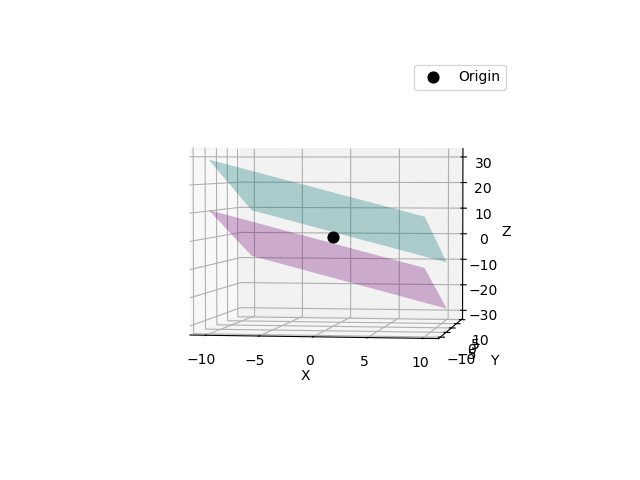
\includegraphics[width=0.9\columnwidth]{figs/fig71.png}
    \caption{}
    \label{fig:placeholder}
\end{figure}
\begin{figure}
    \centering
    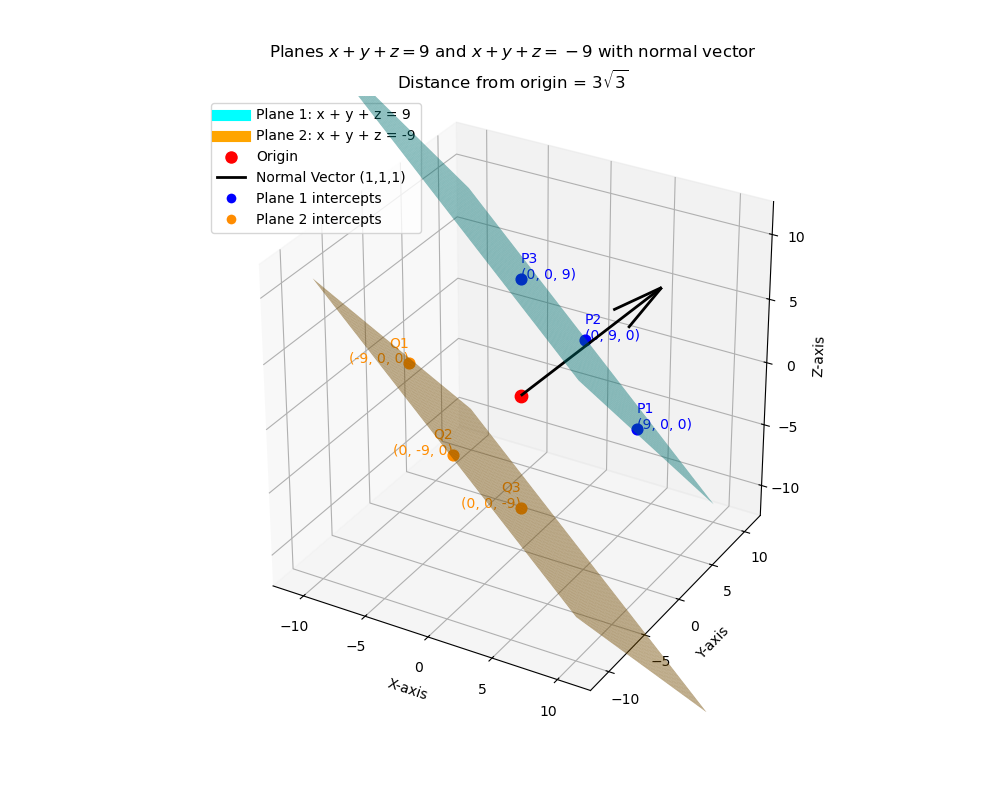
\includegraphics[width=0.9\columnwidth]{figs/fig72.png}
    \caption{}
    \label{fig:placeholder}
\end{figure}
\end{document}